\documentclass[10pt]{article}

\usepackage[paperwidth=192mm
  ,paperheight=108mm
  ,margin=15mm
  ,lmargin=5mm
  ,rmargin=5mm
]{geometry}

\usepackage{amsmath}
\usepackage{fancyhdr}
\usepackage{soul}
\usepackage[utf8]{inputenc}
\usepackage[dvipsnames]{xcolor}

\newcommand{\mydate}{April 27th, 2026}

\fancyhf{}
\renewcommand{\headrulewidth}{0.3pt}
\renewcommand{\footrulewidth}{0.3pt}
\fancyfoot[R]{\tiny\tt \mydate}
\fancyfoot[L]{\tiny\tt mirko.rahn@itwm.fraunhofer.de, github.com/mrahn/klugc-25}
\fancyhead[L]{\tiny\tt \theslideheading}
\fancyhead[R]{\tiny\tt \thepage\ of \pageref{last}}
\renewcommand{\headwidth}{\textwidth}

\newcommand{\theslideheading}{}
\newcommand{\makeslideheading}[1]{\newpage%
\renewcommand{\theslideheading}{#1}%
{\large\bf #1}\\[1em]%
}

\usepackage{graphicx}
\usepackage{amsmath}
\usepackage{amssymb}
\usepackage{microtype}
\usepackage{fixltx2e}
\usepackage{booktabs}

\usepackage{listings}
\usepackage{url}

\setlength{\tabcolsep}{5pt}
\setlength{\arraycolsep}{5pt}
\setlength{\cmidrulekern}{4pt}

\parindent 0pt

\newcommand{\NN}{\mathbb{N}}
\newcommand{\POW}{\mathcal{POW}}

\definecolor{commentgreen}{RGB}{2,112,10}
\definecolor{eminence}{RGB}{108,48,130}
\definecolor{weborange}{RGB}{255,165,0}
\definecolor{frenchplum}{RGB}{129,20,83}

\begin{document}
\addtocounter{page}{-1}
\lstset { language=C++
        , columns=fixed
        , basicstyle=\ttfamily\small
        , showstringspaces=false
        , commentstyle=\color{commentgreen}
        , keywordstyle=\color{eminence}
        , stringstyle=\color{red}
        , emph={int,char,double,float,unsigned,void,bool}
        }

\pagestyle{empty}

~

\vfill

\begin{center}
\textbf{\LARGE \fcolorbox{Yellow}{Yellow}{No Magic!}}\\[2em]
{\large To expose complexity helps users and developers.}\\[2em]
A practical Concurrent Queue and How It Can (Or Can’t) Be Implemented Using P0260R19.\\[2em]

{\large KLUGC++, April 27th, 2026}\\[2em]

{\tt mirko.rahn@itwm.fraunhofer.de}\\[1em]
{\tt github.com/mrahn/klugc-25}

\vfill

~
\end{center}


\newpage
\pagestyle{fancy}

\makeslideheading{\fcolorbox{CornflowerBlue}{CornflowerBlue}{What is Magic?}}

\begin{minipage}{0.618\textwidth}
  To hide complexity means to take decisions (too) early.\\[1em]

  \vfill

  \begin{itemize}
  \item[$\blacksquare$] store configuration in home folder
  \item[$\blacksquare$] use detected hardware, use all available cores
  \item[$\blacksquare$] global parameters, parameter heuristics
  \end{itemize}
  \vfill
  \begin{itemize}
  \item[$\checkmark$] dozends of MPI configuration parameters
  \item[$\checkmark$] fftw calibration run
  \item[$\checkmark$] require complete configuration (file)
  \end{itemize}
  \vfill
\end{minipage}
\hfill
\begin{minipage}{0.382\textwidth}
  
\includegraphics[height=0.618\textheight]{uncle_bob_clean_architecture.jpg}
\end{minipage}

\makeslideheading{\fcolorbox{Dandelion}{Dandelion}{Report Progress:} Applications are hierarchical and are composed of multiple tasks}
\begin{center}
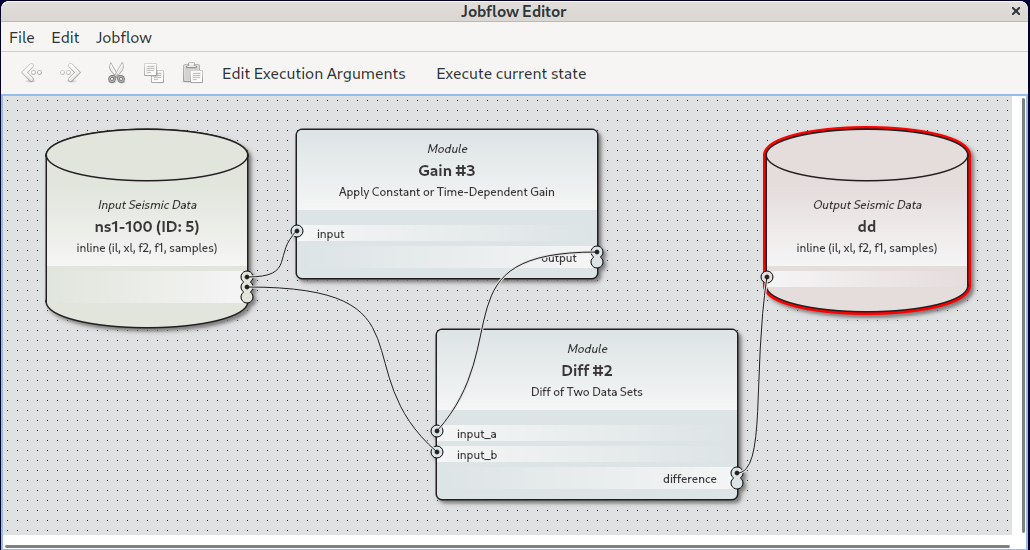
\includegraphics[height=.8\textheight]{aloma_app.png}
\end{center}

\newpage

\begin{center}
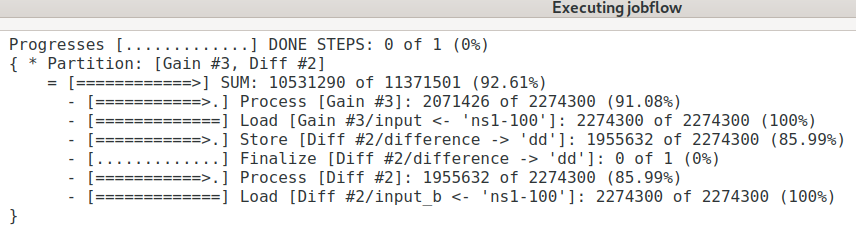
\includegraphics[height=0.618\textheight]{aloma_progress.png}
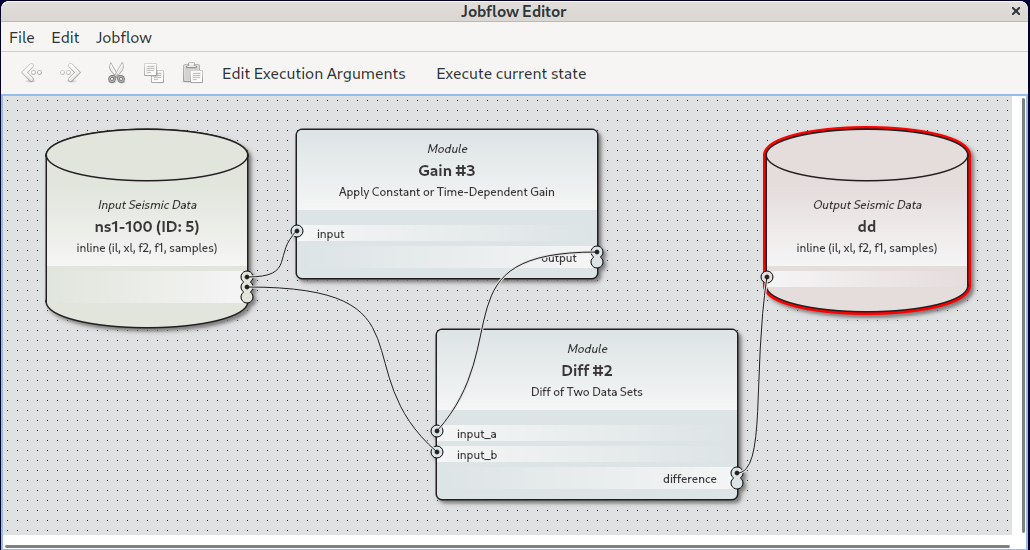
\includegraphics[height=.3\textheight]{aloma_app.png}
\end{center}

\makeslideheading{\fcolorbox{Dandelion}{Dandelion}{Report Status}: Multiple activities happen at the same time}

\begin{center}
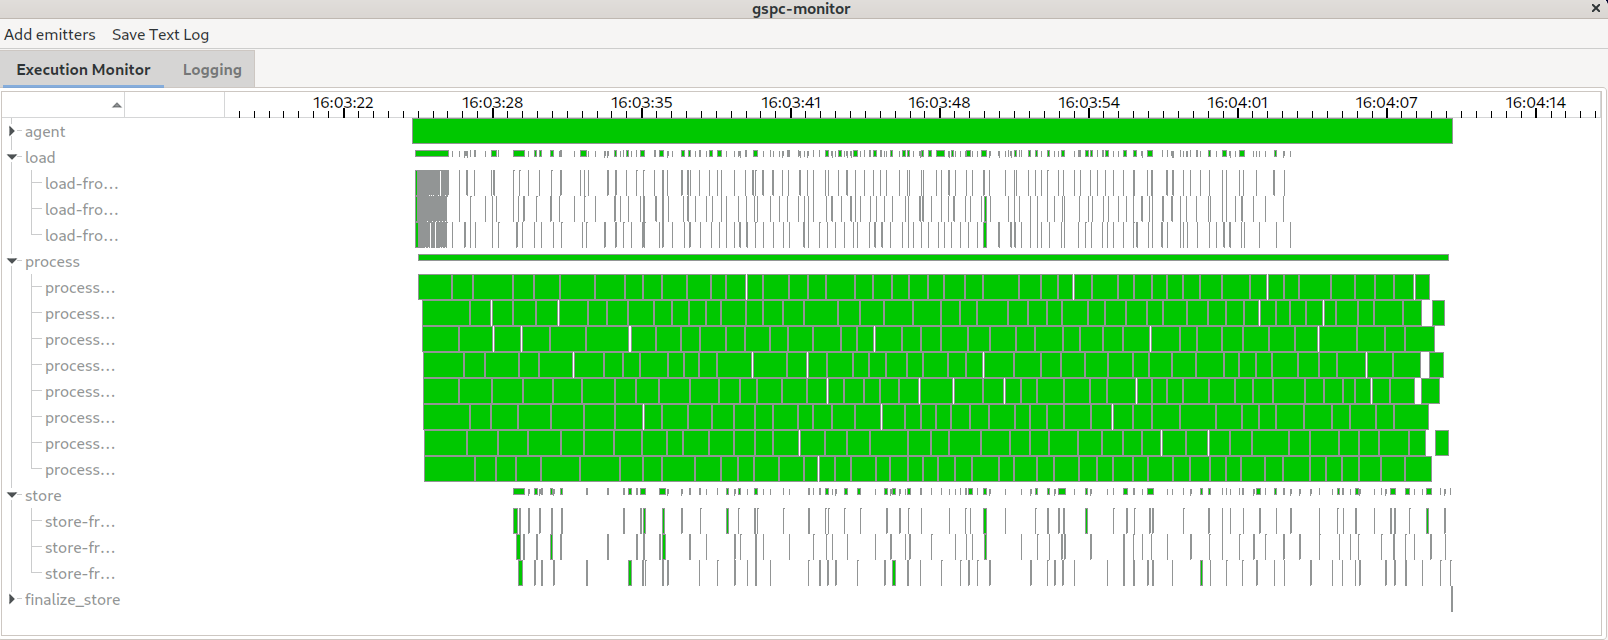
\includegraphics[height=0.8\textheight]{aloma_status.png}
\end{center}

\makeslideheading{\fcolorbox{CornflowerBlue}{CornflowerBlue}{TaskQueue:} Textbook interface, single thread of execution}

\vfill

\begin{minipage}{0.382\textwidth}
\begin{lstlisting}
  class TaskQueue
  {
    auto empty() const -> bool;
    auto push (Task) -> void;
    // pre: !empty()
    auto pop() -> Task;
  }
\end{lstlisting}
\end{minipage}
\begin{minipage}{0.618\textwidth}
\begin{lstlisting}
  tasks.push (root);
single_prosumer:
  while (!tasks.empty())
  {
    auto const task {tasks.pop()};

    for (auto child : execute (task))
    {
      tasks.push (child);
    }
  }
  // FINE
\end{lstlisting}
\end{minipage}

\vfill

\makeslideheading{\fcolorbox{CornflowerBlue}{CornflowerBlue}{TaskQueue:} Textbook interface, single thread of execution}

\vfill

\begin{minipage}{0.382\textwidth}
\begin{lstlisting}
  class TaskQueue
  {
    auto empty() const -> bool;
    auto push (Task) -> void;
    // pre: !empty()
    auto pop() -> Task;
  }
\end{lstlisting}
\end{minipage}
\begin{minipage}{0.618\textwidth}
\begin{lstlisting}
  tasks.push (root);
single_prosumer:
  while (!tasks.empty())
  {
    handle (task.pop());
  }
  // FINE
\end{lstlisting}
\end{minipage}

\vfill

\makeslideheading{\fcolorbox{CornflowerBlue}{CornflowerBlue}{ConcurrentTaskQueue:} Textbook interface, multiple threads of execution}

\vfill

\begin{minipage}{0.382\textwidth}
\begin{lstlisting}
  class ConcurrentTaskQueue
  {
    auto empty() const -> bool;
    auto push (Task) -> void;
    // pre: !empty()
    auto pop() -> Task;
  }
\end{lstlisting}
\end{minipage}
\begin{minipage}{0.618\textwidth}
\begin{lstlisting}
  tasks.push (root);
multiple_prosumers_at_the_same_time:
  while (!tasks.empty())
  {
    handle (tasks.pop()); // PRECONDITION VIOLATION!
  }
\end{lstlisting}
\end{minipage}

\vfill

\makeslideheading{\fcolorbox{CornflowerBlue}{CornflowerBlue}{ConcurrentTaskQueue:} Textbook interface, $k$ many coordinated threads of execution}

\vfill

\begin{minipage}{0.382\textwidth}
\begin{lstlisting}
  class ConcurrentTaskQueue
  {
    // BUMMER! empty() must not exist
    auto empty() const -> bool;
    auto push (Task) -> void;
    // pre: !empty()
    auto pop() -> Task;
  }
\end{lstlisting}
\end{minipage}
\begin{minipage}{0.618\textwidth}
\begin{lstlisting}
  auto done {Atomic {0}};
  tasks.push (root);
k_many_prosumers_at_the_same_time:
  while (done < k)
  {
    if (tasks.empty())
    {
      done += 1;
      while (done < k && tasks.empty()) { yield(); }
    }
    if (!task.empty()))
    {
      done -= 1;
      handle (tasks.pop()); // PRECONDITION VIOLATION!
    }
  }
\end{lstlisting}
\end{minipage}

\vfill

\makeslideheading{\fcolorbox{CornflowerBlue}{CornflowerBlue}{ConcurrentTaskQueue:} pop might return nothing, multiple threads of execution}

\vfill

\begin{minipage}{0.382\textwidth}
\begin{lstlisting}
  class ConcurrentTaskQueue
  {
    auto push (Task) -> void;
    // Nothing if empty
    auto pop() -> optional<Task>;
  }
\end{lstlisting}
\end{minipage}
\begin{minipage}{0.618\textwidth}
\begin{lstlisting}
  tasks.push (root);
multiple_prosumers_at_the_same_time:
  while (auto const task {tasks.pop()})
  {
    handle (*task);
  }
  // BUMMER! ONE THREAD DOES ALL THE WORK!
\end{lstlisting}
\end{minipage}

\vfill

\makeslideheading{\fcolorbox{CornflowerBlue}{CornflowerBlue}{ConcurrentTaskQueue:} Counting client, multiple threads of execution}

\vfill

\begin{minipage}{0.5\textwidth}
\begin{lstlisting}
  class ConcurrentTaskQueue
  {
    struct Client
    {
      auto push (Task) const -> void;
      // Nothing if empty forever
      auto pop() const -> optional<Task>;
    };
    auto client() -> unique<Client>;
  }
\end{lstlisting}
\end{minipage}
\begin{minipage}{0.5\textwidth}
\begin{lstlisting}
  tasks.client()->push (root);
multiple_prosumers_at_the_same_time:
  auto const client {tasks.client()};
  while (auto const task {client->pop()})
  {
    handle (*task);
  }
  // FINE
\end{lstlisting}
\end{minipage}

\vfill

\makeslideheading{\fcolorbox{CornflowerBlue}{CornflowerBlue}{P0260R19:} Relevant API for this talk}

@AI: Please add a slide with a brief summary about the relevant API of P0260.

\vfill

\begin{minipage}{0.55\textwidth}
\begin{lstlisting}
  std::bounded_queue<Task> q {N};

  q.push (task);      // bool
  q.pop();            // optional<Task>

  q.close();          // end-of-stream
  q.is_closed();      // observer

  q.try_push (task);  // conqueue_status
  q.try_pop();        // expected<Task, status>

  q.async_push (task);
  q.async_pop();
\end{lstlisting}
\end{minipage}
\begin{minipage}{0.45\textwidth}
\begin{itemize}
\item No \texttt{empty()}: that would be racy.
\item \texttt{pop()} blocks until data or \texttt{close()}.
\item After \texttt{close()}, queued tasks can still be popped.
\item Once empty and closed, \texttt{pop()} returns \texttt{nullopt}.
\item No standard \texttt{Client}/front/back type in R19.
\item Client counting would have to decide when to call \texttt{close()}.
\end{itemize}
\end{minipage}

\vfill

\makeslideheading{\fcolorbox{CornflowerBlue}{CornflowerBlue}{Quiescence is not Close}}

@AI: Please add a slide ``Quiescence is not Close'' and describe the differences.

\vfill

\begin{minipage}{0.48\textwidth}
\textbf{TaskQueue quiescence}
\begin{itemize}
\item \texttt{pop()} returns nothing if no client can make progress now.
\item This is detected from global state of clients and waiting \texttt{pop()} calls.
\item There is no permanent closed state in the interface.
\item A later \texttt{push()} by an old or new client can start a second round.
\end{itemize}
\end{minipage}
\hfill
\begin{minipage}{0.48\textwidth}
\textbf{P0260 close}
\begin{itemize}
\item \texttt{close()} is explicit and one-way.
\item After \texttt{close()}, every later \texttt{push()} fails.
\item \texttt{pop()} returns nothing only when the queue is empty and closed.
\item No second round on the same queue object is possible.
\end{itemize}
\end{minipage}

\vfill

\makeslideheading{\fcolorbox{CornflowerBlue}{CornflowerBlue}{ConcurrentTaskQueue:} Counting client, multiple threads of execution}

\vfill

\begin{minipage}{0.5\textwidth}
\begin{lstlisting}
  class ConcurrentTaskQueue
  {
    struct Client
    {
      auto push (Task) const -> void;
      //                  +----------+
      // Nothing if empty | FOR EVER |
      //                  +----------+
      auto pop() const -> optional<Task>;
    };
    auto client() -> unique<Client>;
  }
\end{lstlisting}
\end{minipage}
\begin{minipage}{0.5\textwidth}
\begin{lstlisting}
  tasks.client()->push (root);
multiple_prosumers_at_the_same_time:
  auto const client {tasks.client()};
  while (auto const task {client->pop()})
  {
    handle (*task);
  }
  // FINE

  tasks.client()->push (root2);
  // ^BUMMER: Second round interleaves
\end{lstlisting}
\end{minipage}

\vfill

\makeslideheading{\fcolorbox{CornflowerBlue}{CornflowerBlue}{TaskQueue vs Adapter}}

@AI: Please add a slide that summarizes the differences between the TaskQueue and the Adapter.

\vfill

\begin{minipage}{0.48\textwidth}
\textbf{Current TaskQueue}
\begin{itemize}
\item Owns \texttt{deque}, mutex, condition variable, and close state.
\item Decides quiescence directly inside \texttt{pop()}.
\item Wakes blocked clients directly when closing.
\item Queue mechanics and client counting are tightly coupled.
\end{itemize}
\end{minipage}
\hfill
\begin{minipage}{0.48\textwidth}
\textbf{P0260-based Adapter}
\begin{itemize}
\item Underlying queue owns blocking \texttt{pop()}, \texttt{close()}, and wakeup.
\item Adapter keeps only client-aware counters and quiescence logic.
\item Quiescence is translated into one call to \texttt{q.close()}.
\item Most queue machinery moves from the wrapper into the P0260 queue.
\end{itemize}
\end{minipage}

\vfill

\begin{center}
P0260 carries most of the queue machinery,\
the adapter adds only the client-based termination rule.
\end{center}

\vfill

\makeslideheading{\fcolorbox{Yellow}{Yellow}{No Magic!}}
\label{last}

\begin{itemize}
\item Requires that users know what they do.
\item Requires that developers know what they do.
\item \fcolorbox{YellowGreen}{YellowGreen}{Helps users} to know what they do.
\item \fcolorbox{YellowGreen}{YellowGreen}{Helps developers} to know what they do.
\item Leads to \fcolorbox{YellowGreen}{YellowGreen}{better users experience}, short term and long term.
\item Leads to \fcolorbox{YellowGreen}{YellowGreen}{simpler codes}, short term and long term.
\item AI: P0260 carries most queue mechanics, while client-based termination stays explicit in the adapter.
\end{itemize}

\end{document}
